\documentclass[tikz, border = 5pt]{standalone}

\begin{document}
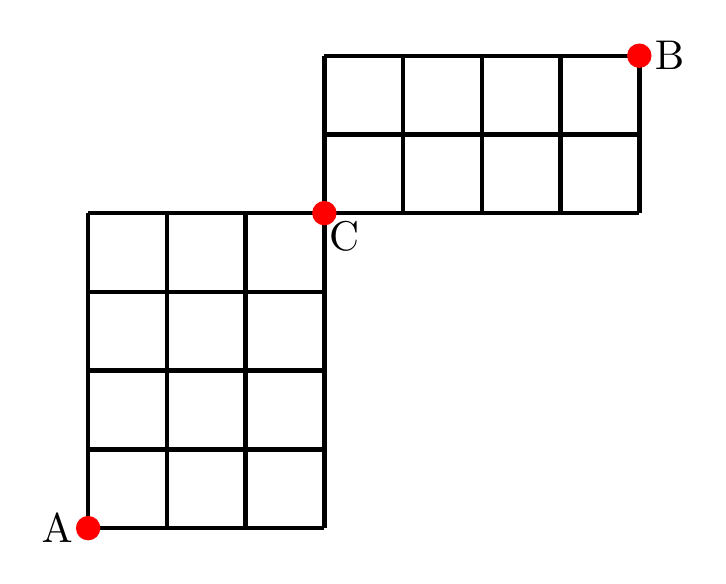
\begin{tikzpicture}

% grid
\draw[ultra thick, step = 1cm] (0, 0) grid (3, 4);
\draw[ultra thick, step = 1cm] (3, 4) grid (7, 6);

\draw [draw=red, fill=red, thick] (0,0) circle (4.0pt) node[scale=1.5, left] {A};
\draw [draw=red, fill=red, thick] (7,6) circle (4.0pt) node[scale=1.5, right] {B};
\draw [draw=red, fill=red, thick] (3,4) circle (4.0pt) node[scale=1.5] at (3.25,3.7) {C};

\end{tikzpicture}
\end{document}
